% Chapter 3

\chapter{Features {\&} Usage}

\label{ch:features}

%----------------------------------------------------------------------------------------

\section{Introduction}\label{sec:features:introduction}

Tangible is a Python library to convert data into tangible 3D models. It
generates code for different backends. It is inspired by projects like OpenSCAD
and d3.js\footnote{\url{http://d3js.org/}}.

The Python programming language\footnote{\url{http://www.python.org/}} has
proven to be an easy, accessible and at the same time very powerful language for
data analysis and many other tasks. Due to its readable syntax, it's very easy
to get started with it, even for people without any prior programming knowledge.
\tangible{} tries to built upon this foundation, by providing an easy to use
software library that has ``batteries included''. It should be easy to process a
dataset, normalize the values and generate the desired visualization.

The difference from Projects like SolidPython is that Tangible is a modular
system with an intermediate representation of objects that is capable of
generating code for different backends, it's not tied to a single
representation. Additionally, its main focus is not general CAD, but printable
3D visualization of data.

Besides the support for model generation and different backends, \tangible{}
also provides utilities to preprocess data, e.g. for normalization of data or
for grouping and aggregation of data.

The library runs on Python 2.6 and 2.7. Support for Python 3.3+ is planned.

%----------------------------------------------------------------------------------------

\section{Usage}\label{sec:features:usage}

\tangible{} was designed to be very straightforward to use. Common data
visualizations should be possible with just a few lines of code.

Visualizing data with \tangible{} consists of three steps: Preprocessing the
data, creating a shape instance and finally rendering the code using the desired
backend.

\subsection{Preprocess Data}

Many times the data is not yet in the right form for visualization. Let's say
that the user has air temperature measurements from every hour during an entire
day. The temperature range is between 8\si{\degree}C during the night and
22\si{\degree}C during the day.

\vspace{.5\baselineskip}
\begin{pythoncode}
>>> temperatures = [
>>>     10, 9, 8, 8, 9, 8, 9, 10, 12, 15, 17, 19,
>>>     20, 22, 22, 21, 20, 17, 14, 12, 11, 10, 9, 10
>>> ]
\end{pythoncode}

\noindent To visualize the data, the user wants to create a round tower where
the radius of a slice corresponds to a temperature measurement. But the
temperatures are not well suited to be used directly as millimeter values.
Therefore the user wants to linearly transform the range 8--22 (\si{\degree}C)
to the range 10--40 (mm).

\tangible{} provides helper functions for this called \emph{scales}. First a
linear scale needs to be constructed:

\vspace{.5\baselineskip}
\begin{pythoncode}
>>> from tangible import scales
>>> scale = scales.linear(domain=[8, 22], codomain=[10, 40])
\end{pythoncode}

\noindent The returned object is the actual scaling function. It can be used directly:

\vspace{.5\baselineskip}
\begin{pythoncode}
>>> scale(8)
10.0
>>> scale(15)
25.0
>>> scale(22)
40.0
\end{pythoncode}

\noindent ...or it can be used in combination with Python's \texttt{map()}
function:

\vspace{.5\baselineskip}
\begin{pythoncode}
>>> radii = map(scale, temperatures)
>>> radii
[14.285714285714285, 12.142857142857142, 10.0, 10.0, ...]
\end{pythoncode}

\noindent Now the data is ready to be visualized. There are also several other
functions to preprocess data, for example to group or aggregate datapoints. For
more information, take a look at section \ref{sec:architecture:utils}
\hyperref[sec:architecture:utils]{Utils}.

\subsection{Create a Shape Instance}

\tangible{} provides many predefined shapes that can be used directly. Currently
there are three types of shapes: Vertical shapes, bar shapes and pie shapes.

For the temperature tower, the user wants the \texttt{CircleTower1D} shape from
the \texttt{tangible.shapes.vertical} module. The class requires two arguments:
The data list as well as the height of each layer.

\vspace{.5\baselineskip}
\begin{pythoncode}
>>> from tangible.shapes.vertical import CircleTower1D
>>> tower = CircleTower1D(data=radii, layer_height=2)
\end{pythoncode}

TODO reference to list of all shapes

\subsection{Render the Code}

Now the shape is ready to be rendered. First, choose the desired backend from
the \texttt{tangible.backends} package. At the time of this writing, the only
available backend is the OpenSCAD backend.

\vspace{.5\baselineskip}
\begin{pythoncode}
>>> from tangible.backends.openscad import OpenScadBackend
\end{pythoncode}

\noindent Next, render the shape using this backend. For convenience, we write
the resulting code into a file.

\vspace{.5\baselineskip}
\begin{pythoncode}
>>> with open('tower.scad', 'w') as f:
...     code = tower.render(backend=openscad.OpenScadBackend)
...     f.write(code)
\end{pythoncode}

\noindent The OpenSCAD code can now be rendered on the command line (or
alternatively from the GUI tool) into an image for previewing or into an STL
file for printing:

\vspace{.5\baselineskip}
\begin{minted}[bgcolor=tango-bg,frame=lines,framesep=2mm,samepage=true,fontsize=\footnotesize]{bash}
$ openscad -o tower.png --render --imgsize=512,512 tower.scad
CGAL Cache insert: cylinder($fn=0,$fa=12,$fs=2,h=5,r1=14.28)
CGAL Cache insert: cylinder($fn=0,$fa=12,$fs=2,h=5,r1=12.14)
...
$ openscad -o tower.stl --render tower.scad
CGAL Cache insert: cylinder($fn=0,$fa=12,$fs=2,h=5,r1=14.28)
CGAL Cache insert: cylinder($fn=0,$fa=12,$fs=2,h=5,r1=12.14)
...
\end{minted}

\noindent The result:

\begin{figure}[H]
	\centering
	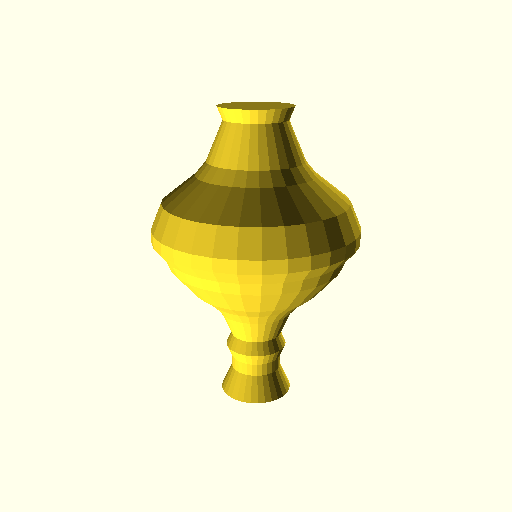
\includegraphics[height=.28\textheight]{images/usage_tower.png}
	\caption{3D visualization of a temperature range}
	\label{img:usage_tower}
\end{figure}

\noindent A few more usage examples are available in the
\hyperref[ch:examples]{Examples} chapter on page \pageref{ch:examples}.

%----------------------------------------------------------------------------------------

\section{Future Developments}\label{sec:features:future}

There are many areas where \tangible{} could still be improved, for example by
adding more backends and shapes, for improving Python version support and by
adding more utils and helper functions.

\subsection{More Backends}

OpenSCAD was chosen as the initial backend because of its popularity. Moreover,
it's freely available and open source. Due to its programmatic nature, it's easy
to implement as a backend and it also allows the resulting code to be modified
directly to make some final adjustments before printing.

Another possible backend would be
ImplicitCAD\footnote{\url{http://www.implicitcad.org/}}. It's a project strongly
inspired by OpenSCAD but withadditional features on top of it. ImplicitCAD is is
written in Haskell and supports both an OpenSCAD compatible "legacy" syntax as
well as the traditional Haskell notation.

Both of these examples are programmatic CAD tools. A step further would be to
support the widely used STL format directly as a backend. But implementing
direct STL generation would have gone beyond the scope of this thesis and was
therefore not attempted.

\subsection{More Shapes}

Right now \tangible{} provides three base shape types with different variants.
But the shape library could be further extended, in order to provide even more
visualizations that can be used by users without any additional modeling
efforts.

\subsection{Interpolation / Smoothing}

\tangible{} provides no tools for interpolation / smoothing of surfaces. This
means that shapes with a lot of datapoints may look verry ragged and printing
them may cause problems because of the overhanging surfaces.

Although libraries like Numpy\footnote{\url{http://www.numpy.org/}} and
SciPy\footnote{\url{http://www.scipy.org/}} provide interpolation functionality,
this is something that \tangible{} should provide out of the box. A possible way
of implementing curve smoothing would be by using spline interpolation. This
feature is planned for a future release.

\subsection{Data Preprocessing Tools}

The current selection of data preprocessing tools is already very useful, but
still doesn't cover many use cases. Therefore these utils should be expanded,
for example by adding logarithmic and exponential scales and by adding more
grouping functions. Furthermore the scales could be improved to allow changes in
the domain / codomain and rescaling the data at any point in time.

\subsection{Python 3 Support}

Right now \tangible{} is written for Python 2.6 / 2.7. But it would be quite
easy add support for Python 3.3+. This is a feature that's already planned and
will be implemented soon.


%----------------------------------------------------------------------------------------
